\section{Results statistics}

To detect the repetibility of the adjustments predicted by the reduction pipeline we select a set of maps taken in the same date to have similar conditions.
For each map we run the complete pipeline and we compare the screws adjustments between the maps. As we dont know the true optimal adjustment, we would only care about the variability of the results.
The maps selected are shown in the figure \ref{fig:statistic_maps} and the figure \ref{fig:hist_example} shows the difference in the screws adjustment heights predicted for different maps that were taken in the same night.

\begin{figure}
    \centering
    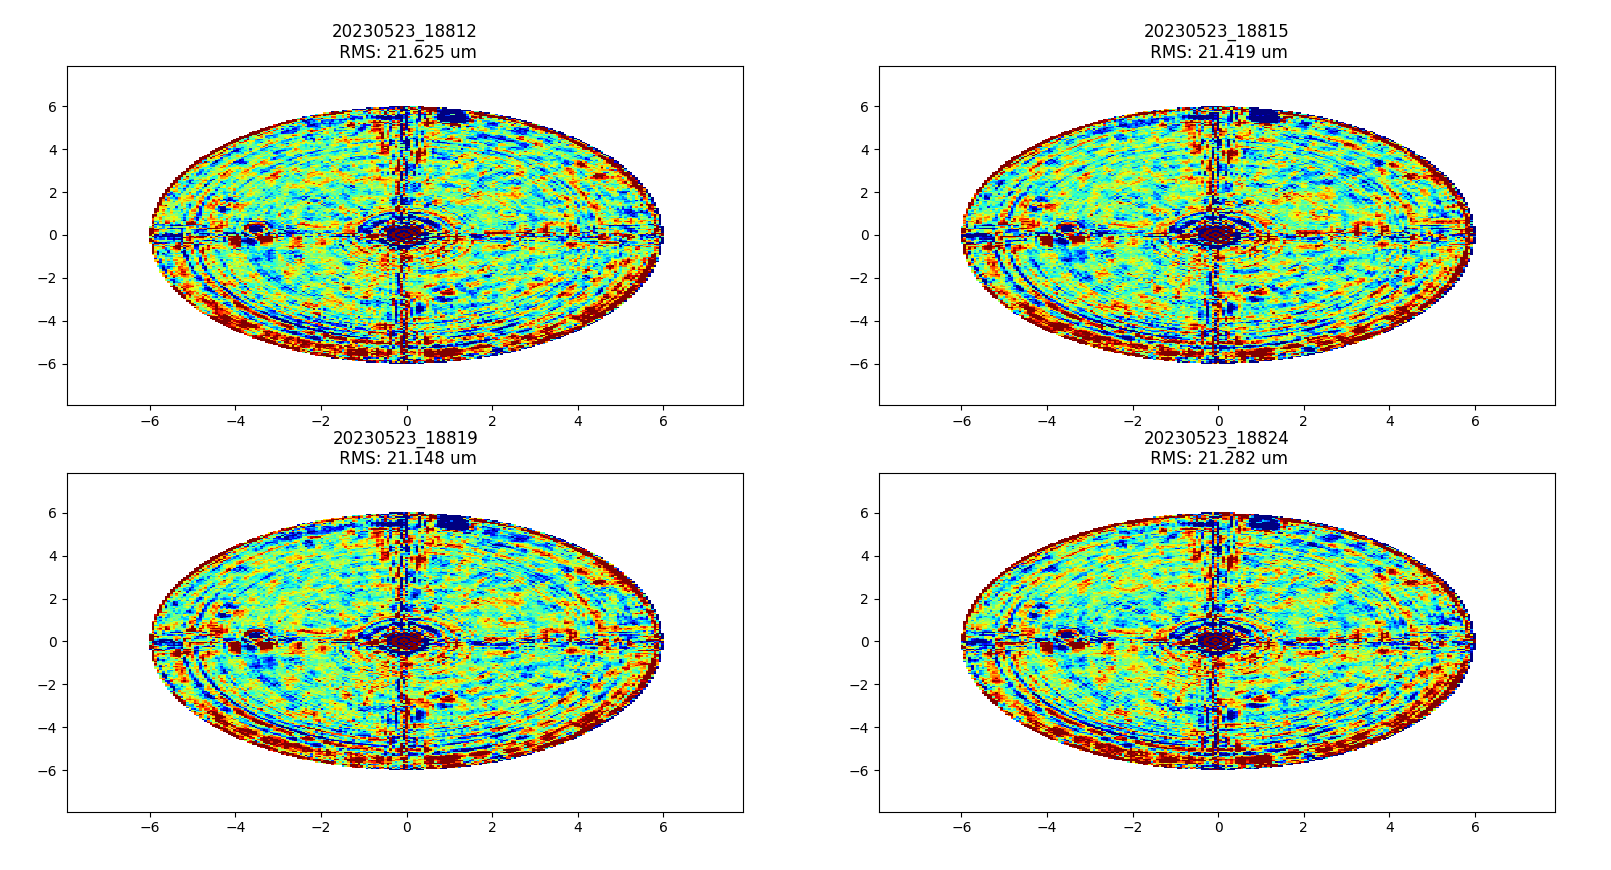
\includegraphics[width=\textwidth]{images/20230523_maps.png}
    \caption{Selected maps for the variability study. These maps are part of a single night measurement, so the conditions when making the maps were comparable.}
    \label{fig:statistic_maps}
\end{figure}



\begin{figure}
    \centering
    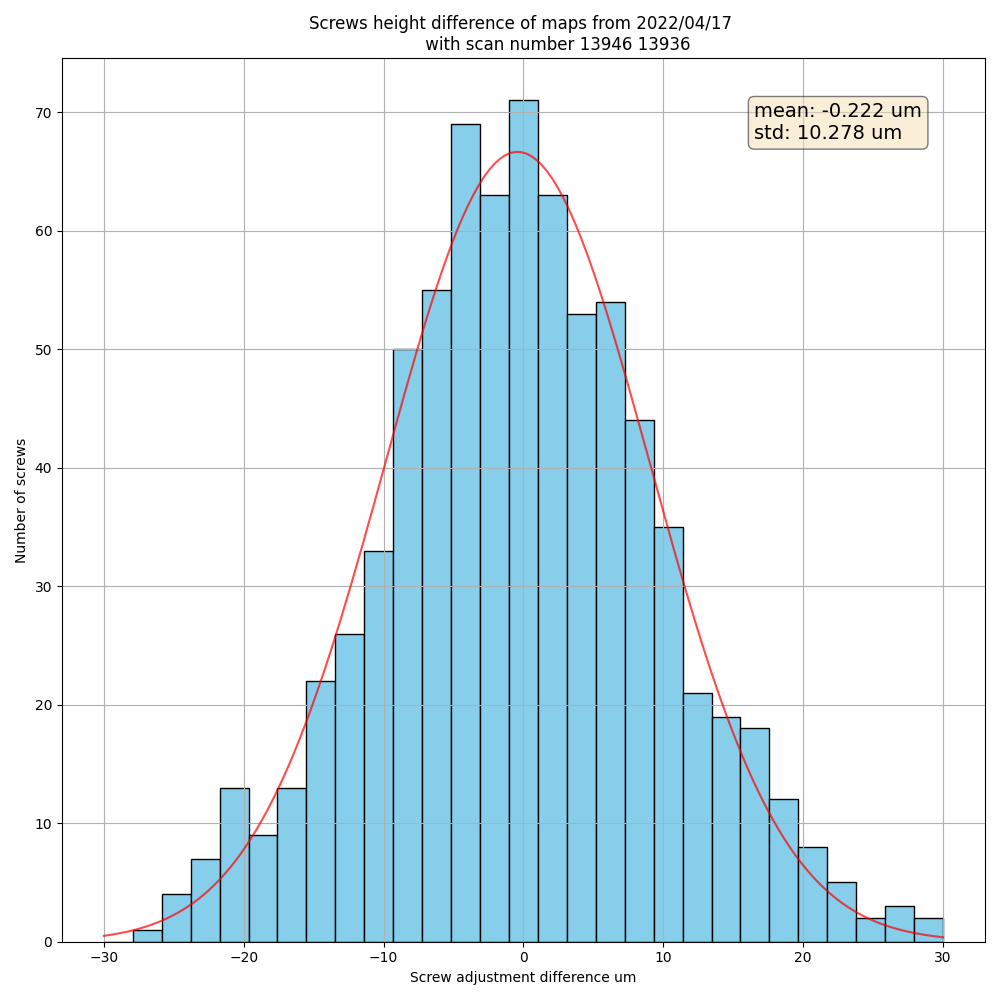
\includegraphics[width=0.6\textwidth]{images/hist_example.png}
    \caption{Example of the obtained histogram when comparing the screws heights values that the pipeline compute for each map.}
    \label{fig:hist_example}
\end{figure}



The histogram plot shows that the difference between the set of screw adjustments can be well represented by a normal distribution where, in a non-rigourous way, the average value can be thoughit as a global piston difference between the two sets and the standard deviation is the measurement variability and its the parameters that we are interested in.

As we do not know the true value of the adjustment we can only make pairwise comparison, considering on of the predictions as true. This can be summarized in the confusion matrix shown in figures \ref{fig:conf_matrix_plane} where for every row the screws adjustment of that map are consider as the true values and compared with the rest maps. Each one of these comparison lead to a distribution like the one shown in figure \ref{hist_example}, the confusion matrix summarize gaussian parameters of every distribution.


The confusion matrix in the figure \ref{fig:conf_matrix_plane} shows the results when using the pure plane panel fitting method, whereas the figure \ref{fig:cong_matrix_deform} use the deformed plane panel fitting.

From these results we can tell that we got a variability around $7-8\mu m$ in the adjustments, so the error that we have in the adjusted surface has that as a lower bound (this is a systematic error, so there are more sources of errorrs, and the final surface error should be higher).


\begin{figure}
    \centering
    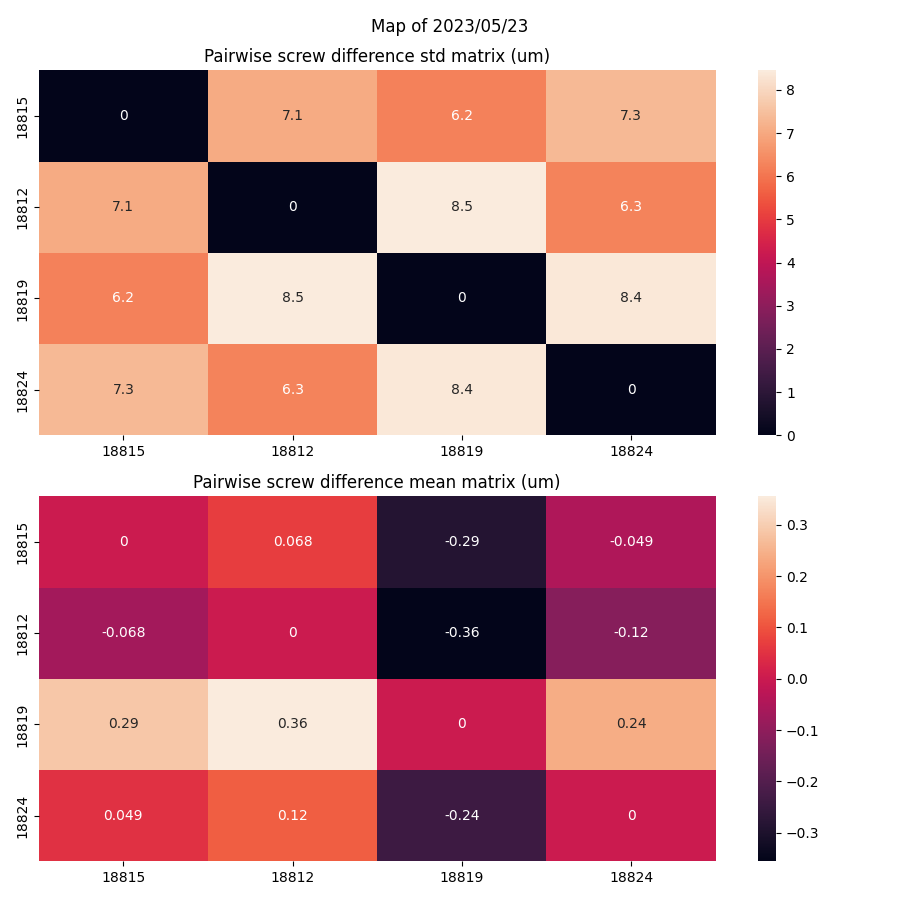
\includegraphics[width=0.8\textwidth]{images/20230523_mat_panelfit_plane.png}
    \caption{Confusion matrix of the maps with the pure plane panel fitting method to compute the screws adjustments.}
    \label{fig:conf_matrix_plane}
\end{figure}

\begin{figure}
    \centering
    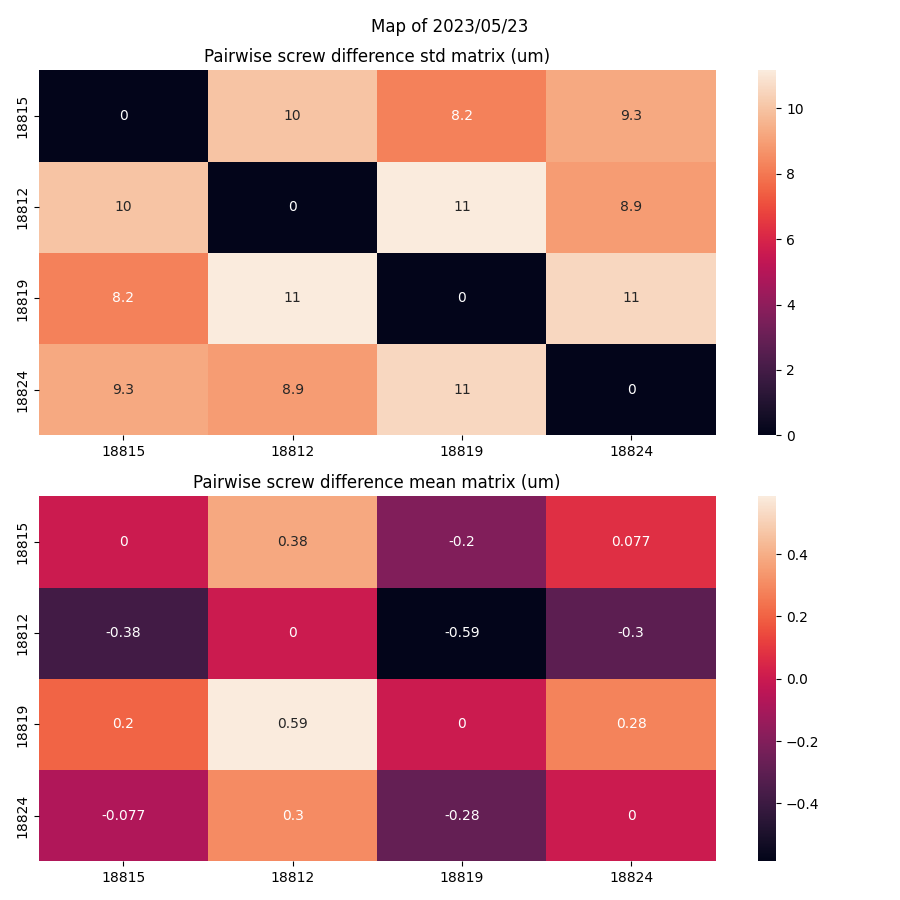
\includegraphics[width=0.8\textwidth]{images/20230523_mat_panelfit_deform.png}
    \caption{Confusion matrix of the maps with the deformed plane panel fitting method to compute the screws adjustments.}
    \label{fig:conf_matrix_deform}
\end{figure}
